\chapter{Comment faire pour ?}
\section{Générer une liste d'échantillons vides}
Objectif : préparer des bocaux d'échantillons avant de partir en campagne de collecte. Ces bocaux doivent être étiquetés.

Le logiciel propose une procédure d'import de masse, qui permet de répondre à cette question.

Voici la méthode à utiliser :
\begin{itemize}
\item générez un fichier au format CSV (créé par exemple à partir de LibreOffice OpenDataSheet -- ODS), qui comprend une ligne par échantillon ;
\item lancez la procédure d'import : le programme vous indiquera les UID générés ;
\item recherchez les UID générés, et déclenchez l'impression des étiquettes.
\end{itemize}

\subsection{Structure du fichier CSV}

Toute opération d'import présente des risques : il est difficile de revenir en arrière une fois celle-ci terminée.
Pour les limiter, le logiciel va procéder en deux étapes. D'abord, la structure du fichier va être analysée, et la cohérence des informations indiquées vérifiée.
Ensuite, si aucune anomalie n'est détectée, l'import pourra être déclenché.

La première ligne du fichier doit comporter le nom des colonnes. Leur nom est normalisé et ne doit en aucun cas être modifié. Si une colonne n'existe pas, l'import du fichier sera rejeté.

Les identifiants numériques (\textit{project\_id} par exemple) doivent être recherchés dans les tables de paramètres de l'application.

Voici la liste des colonnes utilisables :
\begin{longtable}{|p{4cm}|p{8cm}| c|}
\hline
\textbf{Colonne} & \textbf{Description} & \textbf{Obligatoire} \\
\hline
\endhead
sample\_identifier & identifiant métier de l'échantillon & X \\
\hline
collection\_id & identifiant de la collection de rattachement & X \\
\hline
sample\_type\_id & identifiant du type d'échantillon & X \\
\hline
sample\_status\_id & identifiant du statut à attribuer & X \\
\hline
sampling\_place\_id & le numéro informatique de l'endroit où l'échantillon a été prélevé & \\
\hline
wgs84\_x & longitude GPS en WGS84 (degrés décimaux) & \\
\hline
wgs84\_y & latitude GPS en WGS84 (degrés décimaux) & \\
\hline
sampling\_date & date de création/échantillonnage de l'échantillon, au format dd/mm/yyyy & \\
\hline
expiration\_date & date d'expiration de l'échantillon, au format dd/mm/yyyy & \\
\hline
sample\_location & emplacement de rangement de l'échantillon dans le container (texte libre) & \\
\hline
sample\_column & n° de la colonne de stockage dans le container & \\
\hline
sample\_line & n° de la ligne de stockage dans le container & \\
\hline
sample\_multiple\_value & le nombre total de sous-échantillons (ou le volume total, ou le pourcentage...) contenu dans l'échantillon si le type d'échantillons utilisé le permet (valeur numérique, séparateur décimal : point) & \\
\hline
sample\_parent\_uid & UID du parent (création d'échantillons rattachés) &\\
\hline
sample\_metadata\_json & métadonnées rattachées à l'échantillon (au format json, p. e. : \{"taxon":"Alosa alosa"\}) & \\
\hline
container\_identifier & identifiant du container & X \\
\hline
container\_type\_id & identifiant du type de container & X \\
\hline
container\_status\_id & identifiant du statut à attribuer au container & \\
\hline
container\_column & n° de la colonne de stockage dans le container parent & \\
\hline
container\_line & n° de la ligne de stockage dans le container parent & \\
\hline
container\_parent\_uid & UID du container dans lequel le container courant est rangé & \\
\hline
identifiants complémentaires & une colonne par code supplémentaire (menu \textit{Paramètres $\rightarrow$ Types d'identifiants}) & \\
\hline

\caption{Liste des colonnes utilisables lors d'un import de masse}
\end{longtable}

Les champs obligatoires ne le sont que si l'identifiant de l'objet considéré -- échantillon ou container -- a été renseigné. Une ligne doit contenir au minimum soit un numéro d'échantillon, soit un numéro de container.

\subsection{Procédure d'import}

À partir du menu, choisissez \textit{Objet $\rightarrow$ import de masse}. Seuls les utilisateurs qui disposent du droit \textit{projet} ou \textit{import} pourront réaliser l'opération.
\begin{figure}[H]
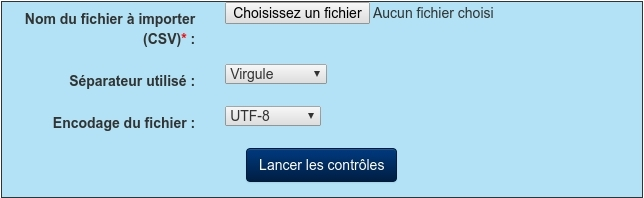
\includegraphics[width=\linewidth]{images/import_controle}
\caption{Sélection du fichier pour un import de masse}
\end{figure}

Sélectionnez le fichier à importer, vérifiez le séparateur utilisé. Préférez, si possible, les données au format UTF-8.

L'import sera réalisé ainsi :
\begin{enumerate}

\item  si sample\_identifier est renseigné : création de l'échantillon
\item    si container\_identifier est renseigné : création du container
\item    si container\_identifier et container\_parent\_uid sont renseignés : création du mouvement d'entrée du container
\item    si l'échantillon et le container ont été créés, création du mouvement d'entrée de l'échantillon dans le container
\item    si l'échantillon est créé, que container\_parent\_uid est renseigné, et que container\_identifier n'est pas rempli, création du mouvement d'entrée de l'échantillon dans le container indiqué

\end{enumerate}

Si des anomalies sont détectées lors du contrôle, un tableau récapitulant les problèmes rencontrés sera affiché, ressemblant à ceci :
\begin{figure}[H]
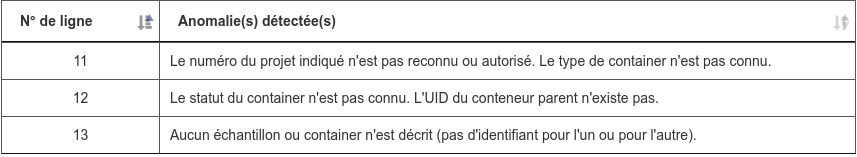
\includegraphics[width=\linewidth]{images/import_tableau}
\caption{Exemples d'anomalies détectées lors du contrôle de l'import}
\end{figure}

Si les contrôles se sont bien déroulés, le programme proposera alors de déclencher l'import, et affichera en retour les valeurs \textit{mini} et \textit{maxi} des UID générées.

\subsection{Autre usage}
Cette fonctionnalité peut également être utilisée pour déclencher l'import de listes d'échantillons pré-existants, et de créer automatiquement les mouvements adéquats pour les ranger dans leurs containers de stockage.

\subsection{Exemple de fichier}
\begin{figure}[H]
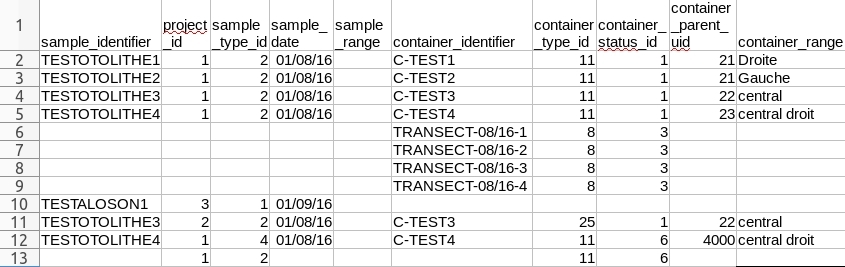
\includegraphics[width=\linewidth]{images/importcsv}
\caption{Exemple d'un fichier CSV}
\end{figure}

Dans cet exemple, l'import ne sera pas réalisé pour les raisons suivantes :
\begin{itemize}
\item en ligne 12, le numéro de container n'existe pas ;
\item la ligne 13 ne contient ni numéro d'échantillon, ni de numéro de container.
\end{itemize}

Sans tenir compte des erreurs, voici les opérations qui seraient exécutées :
\begin{itemize}
\item lignes 2 à 5, 11 et 12 : création d'échantillons, avec création du mouvement d'entrée dans les containers correspondants ;
\item lignes 6 à 9 : création de containers ;
\item ligne 10 : création d'un échantillon non rangé ;
\end{itemize}

\section{Export de données au format JSON}

Il est possible d'exporter un lot de données, réparties sur plusieurs tables, pour les réimporter dans une autre base de données. Par défaut, l'export \og technique\fg{} des modèles d'exports est disponible.

Les données sont exportées au format JSON.

\subsection{Description des modèles d'export}

Choisissez le menu \textit{Paramètres > Modèles d'export}. Hormis le nom du modèle, toutes les autres informations permettent de décrire les tables à exporter et les relations entre elles.

La saisie d'une nouvelle table passe par l'ajout d'un nouvel item dans la partie \textit{Description du modèle}. Chaque item peut être déplacé après création, si nécessaire.

Pour chaque table à exporter, voici les informations à renseigner :
\begin{itemize}
	\item nom de la table, telle qu'il figure dans la base de données
	\item alias de la table : si une même table peut être reliée à des tables parentes différentes, cette colonne devra être renseignée avec un nom différent pour chaque instance. 
	\item  clé primaire : indiquez la clé primaire utilisée dans la table. Elle ne doit pas être renseignée dans le cas d'une table porteuse d'une relation n-n, dont la clé est composée des clés des deux tables parentes.
	\item clé métier : il s'agit de la colonne qui permet de retrouver de manière univoque un enregistrement dans la table. Selon les cas de figure, il peut s'agir :
	\begin{itemize}
		\item du libellé, pour une table de paramètres
		\item de la clé primaire elle-même, pour certaines tables de paramètres dont la clé est significative. Cela permet de conserver la valeur de cette clé, même si le libellé change
		\item du champ UUID, qui est un identifiant technique généré avec un algorithme garantissant qu'il est unique au niveau mondial. Cette valeur sera utilisée chaque fois qu'elle est disponible
	\end{itemize}
	\item clé étrangère : le nom du champ porteur de la relation avec le parent, qui contient donc la clé du parent
	\item la liste des champs de type booléen, en raison d'une particularité lors des importations liée à ceux-ci
	\item la liste des alias (ou du nom des tables) des tables filles
	\item dans le cas d'une table porteuse d'une relation n-n, c'est à dire dont la clé est composée des clés des deux tables parentes, il faudra indiquer :
	\begin{itemize}
		\item le nom du champ comprenant la seconde clé étrangère
		\item l'alias (ou le nom de la table) de la seconde table parente
	\end{itemize}
\end{itemize}

La première table présente dans la liste doit être la table principale de l'export. Les tables filles doivent être créées après leurs tables parentes.

Il est possible d'indiquer plusieurs tables principales (sans parents) dans le même modèle.

\subsection{Importer un fichier JSON}

Il est possible de réaliser une importation rapide depuis le menu de création des modèles d'exportation, depuis le détail d'un modèle. Cette fonction peut être pratique pour mettre à jour des tables de référence.
